\section{入力変数の検討}
\label{sec:input}

\subsection{使用したデータの説明}
本研究で使用したデータは、2016明治安田生命J1リーグ1stステージ第1節の計9試合に関して、
1/30秒毎にパスやタックルなどボール周辺で発生したイベントおよびその発生時刻と位置を取得したボールタッチデータと、1/25秒毎に選手及び審判のピッチ上での位置を取得したトラッキングデータの2種類である。
なお、これらのデータはデータスタジアム株式会社から提供を受けたものである。

\begin{figure*}[t]
  \begin{center} %センタリングする
    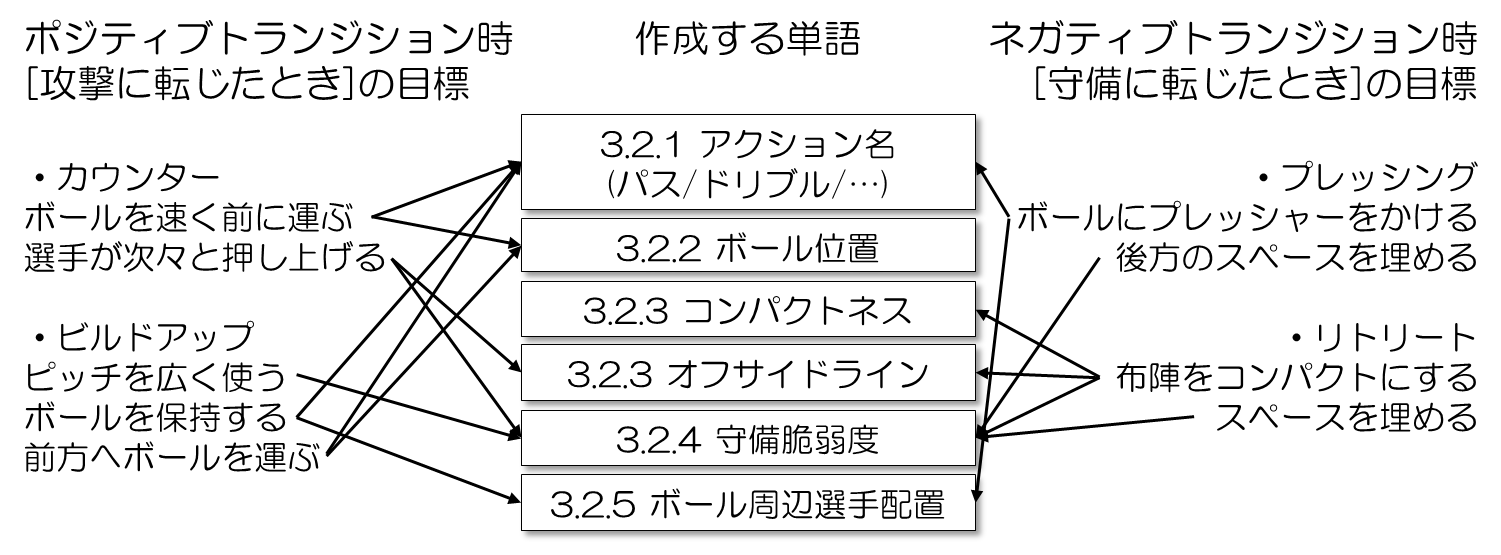
\includegraphics[width=12cm]{img/flow.png}
    %\renewcommand{\baselinestretch}{1}%
    \caption{サッカーの攻防の要素とそれを表す単語の作成}
    \label{fig:flow} %ラベルをつけ図の参照を可能にする
  \end{center}
\end{figure*}

\subsection{単語の作成}
LDAの適用のために、ボールタッチデータから本研究で用いる単語を作成する必要がある。
ここでの目標は、サッカーの一連の攻撃で発生している複雑な動きを、なるべく端的な単語の羅列で表現することである。そして、作成された単語を並べた文をみれば、人やボールの時系列の移動やその順序が表現される状態を目指す。
サッカーの一連の攻撃において実際に生起している事象をもとに検討し(図 \ref{fig:flow})、以下の5種類を作成することとした。



\begin{figure*}[htbp]
  \begin{center} %センタリングする
    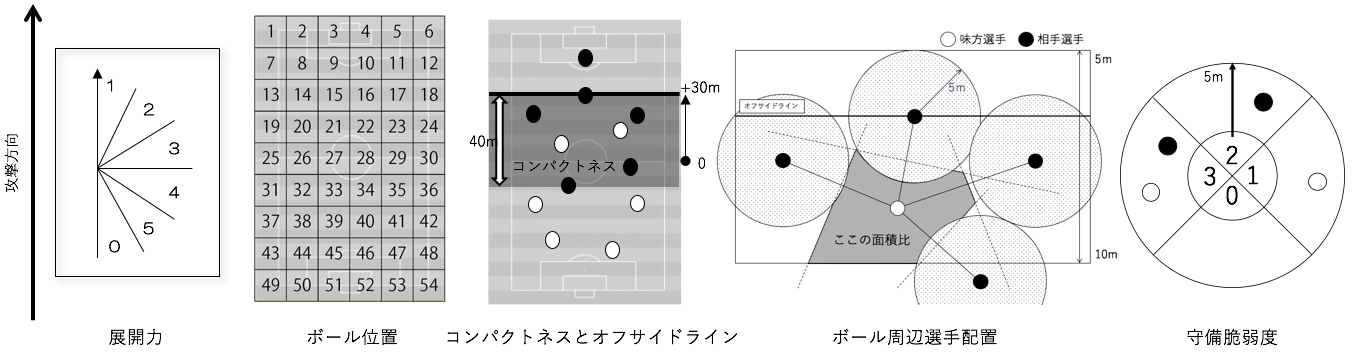
\includegraphics[width=18cm]{img/word.png}
    \renewcommand{\baselinestretch}{1}%
    \caption{作成した単語の例}
    \label{fig:word}
  \end{center}
\end{figure*}

\subsubsection{アクション名}
プレー内容を表現する単語として、ボールタッチデータに整理されている「アクション名」を選定した。
もともとはシュート、パス、GK、フィードなどの単語から構成されている。
ただし、「ホームパス」、「アウェイパス」および「トラップ」の出現回数が他の単語と比較してかなり多く、 特徴的な単語となりにくい可能性がある。
そこで、パスまたはトラップの向きとそのアクションが成功か否かを組み合わせたものをひとつの単語とする。
具体的には、提供されたデータ中の「展開力」と「成功F」を利用した。
例えば、
「パス」のアクションで、「展開力」が1方向、かつ成功の場合、生成される単語は「Pass\_1\_1」となる。
なお、一連の攻撃中に行われる守備側のアクションはすべて「defenseAction」という単語として統一した。


\subsubsection{ボール位置}
ピッチ上を54分割した上で、ボール位置を離散的に表現した単語を作成した。
これは、提供データ中の「hotzone6-9」と同義である。
図\ref{fig:word}にその定義を示す。


\subsubsection{コンパクトネスとオフサイドライン}
ピッチ上の選手配置として考えられる指標として、「コンパクトネス」および「オフサイドライン」を統合した単語を作成する。
コンパクトネスについて本研究では、「一番前方に存在する選手の$X$座標」と「後方より2番目に存在する選手の$X$座標」の距離をコンパクトネスと定義する。
各チームの選手がその時刻において、どれだけピッチ上で展開できているかを示す指標である。
また、オフサイドラインについては「後ろから2人目の選手位置」と定義し、ルール上のオフサイドラインとは異なる点に注意されたい。
この2つの指標は相関をもち、かつ選手がどれくらいの位置・幅でプレーをしているかを表すという点では重複した意味になる可能性がある。
そこで、「コンパクトネス×オフサイドライン」の組み合わせとして単語化することとする。
本研究では、10mずつ離散化して単語化かし、守備側の値のみを利用する。 

\subsubsection{守備脆弱度}
ピッチ上の選手配置のもうひとつの指標として、チームの守備力の脆弱性を表す単語を採用する。
ここでは自陣の最終ライン付近において相手選手が侵入している程度を守備脆弱度と定義する。
具体的には図\ref{fig:word}に示すように、「自軍のオフサイドラインより前方10m、後方5mの長方形のうち、最寄りの味方選手から5m以上離れており、最近傍選手が相手選手であるような地点の合計面積の割合」である。
こちらも守備側の配置のみを文章中の単語として利用する。

\subsubsection{ボール周辺選手配置}
ボール周辺に味方選手もしくは敵選手がいるかを表す単語として採用する。
ボールを中心に半径5mの円を想定し、4分割した各扇形セルそれぞれに、ボールに関与しているプレイヤーを除き、誰もいない場合は「0」、味方選手のみいる場合は「1」、敵選手のみいる場合は「2」、両方の選手がいる場合は「3」の文字を付加していく。
前・右・左・後の順に一つの単語を生成する。
図\ref{fig:word}に具体例を示す。
なお、(2016, 成塚ら)の分析により、「対戦相手との距離が5m以上近づくと、そこから次第に向きをそろえる傾向が強くなる」とされている\cite{2016nar}。
そこで、本研究でも近傍選手として考慮すべき距離を5mと設定した。






